\documentclass[twoside]{article}
\usepackage{relsize,epsfig,makeidx,amsmath,amsfonts, graphicx}
\usepackage[latin1]{inputenc}
\usepackage{amsmath}
% Hyperlinks in PDF:
\usepackage[colorlinks=true,linkcolor=black,citecolor=black,
    filecolor=black,urlcolor=black,pdfmenubar=true,pdftoolbar=true,
    urlcolor=black,bookmarksdepth=3]{hyperref}

\makeindex

\begin{document}
\title{Wave Equation}
\author{Abushet Wosene Simanesew,\\ Daniel Alexander Mo S\o reide Houshmand,\\ Imran Ali}
\date{\today}
\maketitle
\begin{figure} [h]
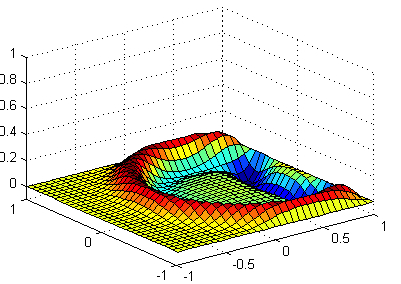
\includegraphics[scale=0.96]{WaveEquation.png}
\caption[A Pretty Wave]{Courtesy of Mathworks}
\end{figure}

\newpage
\tableofcontents

\section{Mathematical Problem}
\label{math:problem}
\index{model problem}\index{exponential decay}

We address the initial-value problem
\begin{align}
\frac{\partial^2u}{\partial t^2} +b\frac{\partial u}{\partial t}  &= \frac{\partial}{\partial x}\left(q(x,y)\frac{\partial u}{\partial x} \right) \\
			  &+\frac{\partial}{\partial y}\left(q(x,y)\frac{\partial u}{\partial y} \right)
		          + f(x,y,t), \quad t \in (0,T], \label{ode} \\
		u(x,y,0)  &= I, \label{initial:value}  \text{ on } \partial \Omega \\
		 \frac{\partial u}{\partial n} &= 0 \text{ on } \partial \Omega \label{eqn:boundaries}
\end{align}
in a rectangular spatial mesh domain $\Omega = [0, L_x]$x$[0, L_y]$. The initial conditions are
\begin{align}
u(x,y,0)=I(x,y),\label{eqn:initial1}\\
u(x,y,0) =V(x,y),  \label{eqn:initial2}
\end{align} \\
where $b$ is damping coefficient, $q(x,y)$ is the square of wave velocity, $T$ the total period and $u(x,y,t)$ is the unknown function to be estimated. This mathematical model addresses the two-dimensional, linear wave equation with damping.

\section{Descretization}
\label{descretization}
\index{mesh in time} \index{$\theta$-rule} \index{numerical scheme}
\index{finite difference scheme}

\subsection{Descritizing the domain}
\label{descritizing the domain}

The temporal domain $[0,T]$ is represented by a finite number of mesh points
\begin{equation}
 0= t_0< t_1 \cdots < t_{N_t+1}=T.
\label{eqn:tdomain}
\end{equation}
Similarly the 2D spatial domain $\Omega = [0, L_x]x[0, L_y]$ is replaced by spatial mesh points
\begin{align}
0 &= x_0< x_1 \cdots <x_{N_x-1}< x_{N_x+1}=L_x,\label{eqn:xmesh}\\
0 &= y_0< y_1 \cdots <y_{N_y-1}< y_{N_y+1}=L_y,  \label{eqn:initial2}
\end{align}
The mesh points are defined as $(x_i,y_j,t_n)$, with indices $i=0, \dots,N_x+1$, $y_j=0, \dots, N_y+1$ and $n=0, \dots, N_t+1$. For uniformly distributed mesh points one can introduce constant mesh spacings $\Delta t$, $\Delta x$ and $\Delta y$, such that the mesh points can be written as follows
 
\begin{align}
x_i=i \Delta x, i=0, \dots,N_x+1,\label{eqn:xmeshp}\\
y_j=i \Delta y, j=0, \dots,N_y+1,\label{eqn:ymeshp}\\
t_n=n \Delta t, n=0, \dots,N_t+1,\label{eqn:tmeshp}
\end{align}

\subsection{The discrete solution}
\label{the discrete solution}

The exact solution $u(x,y,t)$ is now to be approximated by the mesh function $u_{i,j}^{n}$ at the mesh points $(x_i,y_j,t_n)$ defined in the domain above. The numerical solution of the partial differential equation (\ref{ode}) is fulfilled at the interior mesh points:

\begin{align} \notag
\frac{\partial^2u(x_i,y_j,t_n)}{\partial t^2} +b\frac{\partial u(x_i,y_j,t_n)}{\partial t} &= \frac{\partial}{\partial x}\left(q(x_i,y_j)\frac{\partial u(x_i,y_j,t_n)}{\partial x} \right) \\ \notag
&+\frac{\partial}{\partial y}\left(q(x_i,y_j)\frac{\partial u(x_i,y_j,t_n)}{\partial y} \right)\\                                                                                           &+ f(x_i,y_j,t_n), \quad t \in (0,T], \label{eqn:numerical}
\end{align}
for $i=1,\dots , N_x+1$, $j=1,\dots , N_y+1$ and $n=1 \dots ,N_t$. For $n=0$ we have the initial conditions (\ref{eqn:initial1}) and (\ref{eqn:initial2}) and at the boundaries $i=0, N_x+1$ and $j=0,N_y+1$ we have the boundary condition (\ref{eqn:boundaries}). The first and second order derivatives involved in the equation can now be replaced by finite differences. The second-order time derivative to the left side of the equality sign in equation (\ref{eqn:numerical}) can be replaced by central differences

\begin{equation}
 \frac{\partial^2}{\partial t^2}u(x_{i}, y_{j},t_n)\approx\frac{u_{i,j}^{n+1}-2u_{i,j}^n+u_{i,j}^{n-1}}{\Delta t^2}
\label{eqn:doublt}
\end{equation}
The term containing damping is replaced by centered difference as

\begin{equation}
 b\frac{\partial}{\partial t}u(x_i,y_j,t_n)\approx b\frac{u_{i,j}^{n+1}-u_{i,j}^{n-1}}{2\Delta t}
\label{eqn:damping}
\end{equation}
The derivatives containing the the variable coefficients are replaced by centered difference. The variable coefficient at the center of the mesh are estimated by arithimetic average of the mesh points bounding the center point.

 \begin{equation}
\frac{\partial}{\partial x}(q\frac{\partial u}{\partial x})=\frac{q_{i+1/2,j}\frac{u_{i+1,j}^n-u_{i,j}^n}{\Delta x}-q_{i-1/2,j}\frac{u_{i,j}^n-u_{i-1,j}^n}{\Delta x}}{\Delta x}
\label{eqn:variablex1}
\end{equation}

 \begin{equation}
\frac{\partial}{\partial x}(q\frac{\partial u}{\partial x})=\frac{\frac{1}{2}(q_{i,j}+q_{i+1,j})(u_{i+1,j}^n-u_{i,j}^n)-\frac{1}{2}(q_{i,j}+q_{i-1,j})(u_{i,j}^n-u_{i-1,j}^n)}{\Delta x^2}
\label{eqn:variablex2}
\end{equation}

Similarly

\begin{equation}
\frac{\partial}{\partial y}(q\frac{\partial u}{\partial y})=\frac{\frac{1}{2}(q_{i,j}+q_{i,j+1})(u_{i,j+1}^n-u_{i,j}^n)-\frac{1}{2}(q_{i,j}+q_{i,j-1})(u_{i,j}^n-u_{i,j-1}^n)}{\Delta y^2}
\label{eqn:variabley2}
\end{equation}
Before implementation we gather all the terms to solve for $u_{i,j}^{n+1}$:

\begin{align*}
u_{i,j}^{n+1} &= (1+\frac{\Delta t}{2}b)^{-1}*( (\frac{\Delta t b}{2}-1)u_{i,j}^{n-1}+2 u_{i,j}^n \\
            &\quad +\frac{\Delta t^2}{\Delta x^2} \left( \frac{1}{2}(q_{i,j}+q_{i+1,j})(u_{i+1,j}^n-u_{i,j}^n)-\frac{1}{2}(q_{i,j}+q_{i-1,j})(u_{i,j}^n-u_{i-1,j}^n) \right)\\
            & \quad +\frac{\Delta t^2}{\Delta y^2}\left( \frac{1}{2}(q_{i,j}+q_{i,j+1})(u_{i,j+1}^n-u_{i,j}^n)-\frac{1}{2}(q_{i,j}+q_{i,j-1})(u_{i,j}^n-u_{i,j-1}^n)  \right))
            & +\Delta t^2f_{i,j}^{n}
\end{align*}
When $n=0$, a special formula is used for the the initial condition (\ref{eqn:initial2}). The discretization of the initial condition is then:


\begin{equation}
\frac{\partial}{\partial t}u(x_i,y_j,t_n)\approx \frac{u_{i,j}^1-u_{i,j}^{-1}}{2\Delta t}= V_{i,j}
\rightarrow u_{i,j}^{-1}=u_{i,j}^1-2\Delta t V_{i,j}.
\label{eqn:initialalgor}
\end{equation}
The modified scheme for the first step is found by inserting ($\ref{eqn:initial2}$) into the main scheme:

\begin{align*}
u_{i,j}^{1} &= u_{i,j}^0+((\Delta t-\frac{\Delta t^2 b}{4})V_{i,j} \\
            &\quad +\frac{\Delta t^2}{\Delta x^2} \left( \frac{1}{4}(q_{i,j}+q_{i+1,j})(u_{i+1,j}^0-u_{i,j}^0)-\frac{1}{4}(q_{i,j}+q_{i-1,j})(u_{i,j}^0-u_{i-1,j}^0) \right)\\
            & \quad +\frac{\Delta t^2}{\Delta y^2}\left( \frac{1}{4}(q_{i,j}+q_{i,j+1})(u_{i,j+1}^0-u_{i,j}^0)-\frac{1}{4}(q_{i,j}+q_{i,j-1})(u_{i,j}^0-u_{i,j-1}^0)  \right))
            & +\Delta t^2f_{i,j}^{0}
\end{align*}

\subsection{Discretization of derivatives at the boundary}
\label{boundary2}
Since the main equation is discretized by the centeral difference method, a way to implement the boundary conditions (\ref{eqn:boundaries}) should be devised. At $x=0 (i=0)$ and $y=0 (j=0)$ for $t=t_n$ the difference is written as

\begin{align}
\frac{u_{-1,j}^n-u_{1,j}^n}{2\Delta x} = 0,\quad \rightarrow \quad u_{-1,j}^n = u_{1,j}^n\label{eqn:boundx0}\\
\frac{u_{i,-1}^n-u_{i,1}^n}{2\Delta y} = 0,\quad \rightarrow \quad u_{i,-1}^n = u_{i,1}^n\label{eqn:boundy0}
\end{align}
At the boundaries, the conditions $\frac{\partial q}{\partial x}=0$ and $\frac{\partial q}{\partial y}=0$ are imposed on variable coefficient $q$, to ease the implementation.The corresponding boundary conditions of the scheme for $x=L_x (i=Nx)$ and $y=L_y (j=N_y)$ are respectively

\begin{align}
\frac{u_{N_x+1,j}^n-u_{N_x-1,j}^n}{2\Delta x} = 0,\quad \rightarrow \quad u_{N_x+1,j}^n = u_{N_x-1,j}^n\label{eqn:boundx0}\\
\frac{u_{i,N_y+1}^n-u_{i,N_y-1}^n}{2\Delta y} = 0,\quad \rightarrow \quad u_{i,N_y+1}^n = u_{i,N_y-1}^n\label{eqn:boundy0}
\end{align}
The Neumann boundary condition is implemented by updating ghost cells in the simulation. Part of the code looks as follows

\begin{quote}
\begin{verbatim}
def NeumannBC(self,u,Ix,Iy,version="scalar"):
        if version=="scalar":
            for j in range(0,Iy[-1]+1):
                i = Ix[0] # physical grid point 0
                u[i-1,j] = u[i+1,j] 
                i = Ix[-1] # physical grid point Nx+1
                u[i+1,j] = u[i-1,j]
                
            for i in range(0,Ix[-1]+1):
                j = Iy[0] # physical grid point 0
                u[i,j-1] = u[i,j+1]
                j = Iy[-1] # physical grid point Ny+1
                u[i,j+1] = u[i,j-1]
                        
        elif version=="vectorized":
            i = Ix[0]
            u[i-1,:] = u[i+1,:]
            i = Ix[-1]
            u[i+1,:] = u[i-1,:]
            j = Iy[0]  
            u[:,j-1] = u[:,j+1]
            j = Iy[-1]
            u[:,j+1] = u[:,j-1]
        return u
\end{verbatim}
\end{quote}

%%%%%%%% Section 3 %%%%%%%%%
\section{Truncation Error}

Suppose that we want to measure the closeness with which the polynomial
$P_{n}(x)$ approximates the function $u(t)$. This closeness can
then be measured by the difference 
\[
R_{n}(t)=u(t)-P_{n}(t)
\]
This difference $R_{n}(x)$ is the $n$th-degree remainder for $u(t)$
at $t=a$. It is the error made if the value $u(t)$ is replaced with
the approximation $P_{n}(t)$, and it is called the truncation error.
More spesifically, we have for central difference approximation, equations
on the form: 
\[
R^{n}=[D_{k}u]^{n}-u'(k_{n})
\]
 The common way of calculating $R^{n}$ in a centered difference
scheme is to:
\begin{enumerate}
\item Expand $u(t_{n+\frac{1}{2}})$ and $u(t_{n+\frac{1}{2}})$ in a Taylor
series arround the point $t_{n}$ where the derivative is evaluated.
\item Insert this Taylor series in $R^{n}=[D_{k}u]^{n}-u'(k_{n})$
\item Collect terms that cancel and simplify the expression
\end{enumerate}
The result is an expression for $R^{n}$ in terms of power series
in $\Delta t$. The truncation error is the residual $R$ in the equation
and most of the terms needed in our equation i taken from main\_trunc
and been modified to fit our problem . Showing here term by term calculations. 

\begin{equation}
[D_{t}D_{t}u_{e}+bD_{2t}u_{e}=D_{x}\bar{q}^{x}D_{x}u_{e}+D_{y}\bar{q}^{y}D_{y}u_{e}+f+R]_{i,j}^{n}
\end{equation}
The first term on the left hand side (lhs)

\begin{equation}
[D_{t}D_{t}u_{e}]_{i,j}^{n}=\frac{u^{n+1}-2u^{n}+u^{n-1}}{\Delta t^{2}}=u''(t_{n})+R^{n}
\end{equation}


\begin{equation}
R^{n}=\frac{1}{12}u^{(4)}(t_{n})\Delta t^{2}+O(\Delta t^{4})
\end{equation}
The second term on lhs

\begin{equation}
[D_{2t}u_{e}]_{i,j}^{n}=\frac{u^{n+1}-u^{n-1}}{2\Delta t}=u'(t_{n})+R^{n}
\end{equation}


\begin{equation}
R^{n}=\frac{1}{6}u'''(t_{n})\Delta t^{2}+O(\Delta t^{4})
\end{equation}
The x-term on rhs with variable coefficient

\begin{equation}
[D_{x}\bar{q}^{x}D_{x}u_{e}]_{i+\frac{1}{2},j}^{n}=\frac{1}{\Delta x}\left([\bar{q}^{x}D_{x}u_{e}]_{i+\frac{1}{2},j}^{n}-[\bar{q}^{x}D_{x}u_{e}]_{i-\frac{1}{2},j}^{n}\right)
\end{equation}


\begin{equation}
[D_{x}u_{e}]_{i+\frac{1}{2},j}^{n}=u_{e,x}(x_{i+\frac{1}{2},},y_{j},t_{n})+\frac{1}{24}u_{e,xxx}(x_{i+\frac{1}{2}},y_{j},t_{n})\Delta x^{2}+O(\Delta x^{4})
\end{equation}


\begin{equation}
[\bar{q}^{x}]_{i+\frac{1}{2},j}=q(x_{i+\frac{1}{2},}y_{j})+\frac{1}{8}q''(x_{i+\frac{1}{2},}y_{j})\Delta x^{2}+O(\Delta x^{4})
\end{equation}


\begin{align}
[\bar{q}D_{x}u_{e}]_{i+\frac{1}{2},j}^{n} =& \left[q(x_{i+\frac{1}{2}},y_{j})+\frac{1}{8}q''(x_{i+\frac{1}{2}},y_{j})\Delta x^{2}+O(\Delta x^{4})\right] \cdot\\ \notag
&\left[u_{e,x}(x_{i+\frac{1}{2}},y_{j},t_{n})+\frac{1}{24}u_{e,xxx}(x_{i+\frac{1}{2}},y_{j},t_{n})\Delta x^{2}+O(\Delta x^{4})\right] \\ \notag
%%%%%%%%%%%%%%%%%%%%%%%%%%%
=& \hspace{1mm}q(x_{i+\frac{1}{2}},y_{j},t_{n})u_{e,x}(x_{i+\frac{1}{2}},y_{j},t_{n})+q(x_{i+\frac{1}{2}},y_{j})\frac{1}{24}u_{e,xxx}(x_{i+\frac{1}{2}},y_{j},t_{n})\Delta x^{2}\\ \notag
&+u_{e,x}(x_{i+\frac{1}{2}},y_{j},t_{n})\frac{1}{8}q''(x_{i+\frac{1}{2}},y_{j})\Delta x^{2}+O(\Delta x^{4}) \\ \notag 
%%%%%%%%%%%%%%%%%%%%%%%%%%%
=& \hspace{1mm}[qu_{e,x}]_{i+\frac{1}{2},j}^{n}+G_{i+\frac{1}{2},j}^{n}\Delta x^{2}+O(\Delta x^{4})
\end{align}
with introduction of the short form
\begin{equation*}
G_{i+\frac{1}{2},j}^{n}= \left(\frac{1}{24}u_{e,xxx}(x_{i+\frac{1}{2}},y_{j},t_{n})q(x_{i+\frac{1}{2}},y_{j})+u_{e,x}(x_{i+\frac{1}{2}},y_{j},t_{n})\frac{1}{8}q''(x_{i+\frac{1}{2}},y_{j}) \right)\Delta x^{2} .
\end{equation*}
Similary, we find that
\begin{equation}
[\bar{q}D_{x}u_{e}]_{i-\frac{1}{2},j}^{n}=[qu_{e,x}]_{i-\frac{1}{2},j}^{n}+G_{i-\frac{1}{2},j}^{n}\Delta x^{2}+O(\Delta x^{4})
\end{equation}
Inserting the expression in equation (29)
\begin{align*}
[D_{x}\bar{q}^{x}D_{x}u_{e}]_{i,j}^{n} =&\hspace{1mm}\frac{1}{\Delta x}\left([\bar{q}^{x}D_{x}u_{e}]_{i+\frac{1}{2},j}^{n}-[\bar{q}^{x}D_{x}u_{e}]_{i-\frac{1}{2},j}^{n}\right) \\
%%%%%%%%%%%%%%%%%%%%%%%%%%
=&\hspace{1mm} \frac{1}{\Delta x}[qu_{e,x}]_{i+\frac{1}{2},j}^{n}+G_{i+\frac{1}{2},j}^{n}\Delta x^{2}-[qu_{e,x}]_{i-\frac{1}{2},j}^{n}-G_{i-\frac{1}{2},j}^{n}\Delta x^{2}+O(\Delta x^{4})) \\
%%%%%%%%%%%%%%%%%%%%%%%%%%
=&\hspace{1mm} [D_{x}qu_{e,x}]_{i,j}^{n}+[D_{x}G]_{i,j}^{n}\Delta x^{2}+O(\Delta x^{4})
\end{align*}
\begin{align*}
[D_{x}qu_{e,x}]_{i,j}^{n} \hspace{2mm} =& \frac{\partial}{\partial x}q(x_{i},y_{j})u_{e,x}(x_{i},y_{j},t_{n})+\frac{1}{24}G_{xxxx}(x_{i},y_{j},t_{n})\Delta x^{2}+O(\Delta x^{4}) \\
%%%%%%%%%%%%%%%%%%%%%%%%%%%%%%%
[D_{x}G]_{i,j}^{n}\Delta x^{2} =& G_{x}(x_{i},y_{j},t_{n})\Delta x^{2}+\frac{1}{24}G_{xxx}(x_{i},y_{j},t_{n})\Delta x^{4}+O(\Delta x^{4}) \\
%%%%%%%%%%%%%%%%%%%%%%%%%%%%%%%
[D_{x}\bar{q}^{x}D_{x}u_{e}]_{i,j}^{n} =& \frac{\partial}{\partial x}q(x_{i},y_{j})u_{e,x}(x_{i},y_{j},t_{n})+O(\Delta x^{2})
\end{align*}
Similar procedure for the y-component follows. Writing out the result from
equation (29)
\begin{align*}
[D_{y}\bar{q}^{y}D_{y}u_{y}]_{i,j}^{n} =& \frac{1}{\Delta y}\left([\bar{q}^{y}D_{y}u_{e}]_{i,j+\frac{1}{2}}^{n}-[\bar{q}^{y}D_{y}u_{e}]_{i,j-\frac{1}{2}}^{n}\right) \\
%%%%%%%%%%%%%%%%%%%%%%%%%%%%%%
=& \frac{1}{\Delta y}[qu_{e,y}]_{i+\frac{1}{2},j}^{n}+G_{i+\frac{1}{2},j}^{n}\Delta y^{2}-[qu_{e,y}]_{i-\frac{1}{2},j}^{n}-G_{i-\frac{1}{2},j}^{n}\Delta y^{2}+O(\Delta y^{4})) \\
%%%%%%%%%%%%%%%%%%%%%%%%%%%%%%
=& [D_{y}qu_{e,y}]_{i,j}^{n}+[D_{y}G]_{i,j}^{n}\Delta x^{2}+O(\Delta y^{4})
\end{align*}
%%%%%%%%%%%%%%%%%%
\begin{align*}
[D_{y}qu_{e,y}]_{i,j}^{n} =& \frac{\partial}{\partial y}q(x_{i},y_{j})u_{e,y}(x_{i},y_{j},t_{n})+\frac{1}{24}G_{yyyy}(x_{i},y_{j},t_{n})\Delta y^{2}+O(\Delta y^{2}) \\
%%%%%%%%%%%%%%%%%%
[D_{y}G]_{i,j}^{n}\Delta y^{2} =& G_{y}(x_{i},y_{j},t_{n})\Delta y^{2}+\frac{1}{24}G_{yyy}(x_{i},y_{j},t_{n})\Delta y^{4}+O(\Delta y^{4}) \\
%%%%%%%%%%%%%%%%%%
[D_{y}\bar{q}^{y}D_{y}u_{e}]_{i,j}^{n} =& \frac{\partial}{\partial y}q(x_{i},y_{j})u_{e,y}(x_{i},y_{j},t_{n})+O(\Delta y^{2})
\end{align*}
$\downarrow$ $\downarrow$ $\downarrow$ $\downarrow$ $\downarrow$ $\downarrow$ $\downarrow$ $\downarrow$ $\downarrow$ $\downarrow$ $\downarrow$ $\downarrow$
$\downarrow$ $\downarrow$ $\downarrow$ $\downarrow$ $\downarrow$ $\downarrow$
$\downarrow$ $\downarrow$ $\downarrow$ $\downarrow$ $\downarrow$ $\downarrow$
$\downarrow$ $\downarrow$ $\downarrow$ $\downarrow$ $\downarrow$ $\downarrow$
$\downarrow$ $\downarrow$ $\downarrow$ $\downarrow$ $\downarrow$ $\downarrow$
\begin{align} \notag
R_{i,j}^{n} =& \frac{1}{12}u_{e,tttt}(x_{i},y_{j},t_{n})\Delta t^{2}+O(\Delta t^{4}) +b\left(\frac{1}{6}u'''(t_{n})\Delta t^{2}+O(\Delta t^{4})\right) \\ \notag
%%%%%%%%%%%%%%%%%%%%%%%%%%%%
+& \frac{\partial}{\partial x}q(x_{i},y_{j})u_{e,x}(x_{i},y_{j},t_{n})+O(\Delta x^{2})+\frac{\partial}{\partial y}q(x_{i},y_{j})u_{e,y}(x_{i},y_{j},t_{n})+O(\Delta y^{2}) \\ \notag
+& f(x_{i},y_{j},t_{n}) \\
%%%%%%%%%%%%%%%%%%
=& \Delta t^{2}\left[\left(\frac{1}{12}u_{e,tttt}(x_{i},y_{j},t_{n})\right)+b\left(\frac{1}{6}u'''(t_{n})\right)\right] \\ \notag
%%%%%%%%%%%%%%%%%%
+&\left(\frac{\partial}{\partial x}q(x_{i},y_{j})u_{e,x}(x_{i},y_{j},t_{n})\right)+\left(\frac{\partial}{\partial y}q(x_{i},y_{j})u_{e,y}(x_{i},y_{j},t_{n})\right)  \\ \notag
+& O(\Delta t^{4},\Delta x^{2},\Delta y^{2}) + f(x_{i},y_{j},t_{n})
\end{align}
The error is in second order in space, that is $\Delta x^{2},\Delta y^{2}$, and fourth order in time $\Delta t^{4}$. 



%%%%%%%%%% Section 4 %%%%%%%%%%%%
\section{Verification: Standing Undamped Waves}

Neglecting damping and with constant wave velocity, we can assume
standing wave solution without source term, on the form 
\begin{align}
u_{e}(x,y,t) =& Acos(k_{x}x)cos(k_{y}y)cos(\omega t) \\ \notag
k_{x} =&\frac{m_{x}\pi}{L_{x}} \\ \notag
k_{y} =& \frac{m_{y}\pi}{L_{y}} 
\end{align}
for arbitrary amplitude $A$, arbitrary integers $m_{x}$ and $m_{y}$,
and a suitable choice of $\omega$ the solution can be used to test
the convergence of the numerical method. Even though the truncation
error is not the true error $e_{i,j}^{n}=u_{e}(x_{i},y_{j},t_{n})-u_{i,j}^{n}$,
we can assume that $e_{i,j}^{n}$ depends on th discretization parameters
in the same way. We also assume that a norm $e_{i,j}^{n}$, e.g

\[
E=\Vert e_{i,j}^{n}\Vert_{l^{\infty}}=\underset{i}{max}\hspace{1mm}\underset{j}{max}\hspace{1mm}\underset{t}{max}\hspace{1mm}\mid e_{i,j}\mid
\]
Inserting equation (35) in equation (34) and assuming constant $q$, our truncation
error takes the form 

\begin{align*}
R_{i,j}^{n} =& \frac{1}{12}\left[\left(u_{e,tttt}(x_{i},y_{j},t_{n})\Delta t^{2}\right)+\left(u_{e,xxxx}(x_{i},y_{j},t_{n})\right)+\left(u_{e,yyyy}(x_{i},y_{j},t_{n})\right)\right]\\
%%%%%%%%%%%%%
e_{i,j}^{n} = R_{i,j}^{n} =&\Delta t^{2}\left(\frac{1}{12}\omega^{4}Acos(k_{x}x)cos(k_{y}y)cos(\omega t)\right)+\left(Ak_{x}^{4}cos(k_{x}x)cos(k_{y}y)cos(\omega t)\right) \\
+&\left(Ak_{y}^{4}cos(k_{x}x)cos(k_{y}y)cos(\omega t)\right)
\end{align*}
The norm then takes the form
\[
E=\underset{i}{max}\hspace{1mm}\underset{j}{max}\hspace{1mm}\underset{t}{max}\hspace{1mm}\mid e_{i,j}\mid=\frac{1}{12}\left(\Delta t^{2}\omega^{4}+q(\Delta x^{2}k_{x}^{4}+\Delta y^{2}k_{y}^{4})\right)
\]
and for h  $= \Delta x = \Delta y$, $E = Ch^{2}$.
\\ \\
The following output has been taken from the implementation for the undamped standing wave

\begin{center}
\begin{tabular}{ l | c|c }
h & E/$h^2$& $r$ \\
\hline
&  \\
0.500000 & 0.572456 & --------\\
0.250000 & 1.006119 & 1.186437\\
0.125000 & 0.730571 & 2.461704\\
0.062500 & 0.713948 & 2.033207\\
0.031250 & 0.771668 & 1.887838\\
0.015625 & 0.732676 & 2.074804\\
\end{tabular}
\end{center}
We see that the convergence rate is of order 2, which is what we expected for our implementation. We also see that $E/h^2$ is almost a constant.

%%%%%%%% Section 5 %%%%%%%%%
\section{Verification: Standing Damped Waves}
\index{Verification: Standing, damped waves}

Finding the analytical solution of damped waves using an ansatz of the type

\begin{align}\label{eqn:verificationsdw} 
 u_e(x, y, t) =& (A\cos(\omega t) + B\sin(\omega t))e^{-ct}\cos(k_x x)\cos(k_y y), \\ \notag
 k_x =& \frac{m_x\pi}{L_x}, \quad k_y=\frac{m_y \pi}{L_y}.
\end{align}
The aim is to find $A$, $B$, $\omega$, and $c$ such that (\ref{eqn:verificationsdw}) solves the PDE with constant $q$, no source term and initial condition $u_t(x,y,0)=0$. The first derivative of (\ref{eqn:verificationsdw}) with respect to time is

\begin{equation}
 \frac{\partial u_e}{\partial t} = (-c(A\cos(\omega t)+B\sin(\omega t)) + \omega (-A\sin(\omega t) + B\cos(\omega t))) e^{-ct} \cos (k_x x) \cos(k_y y).
\label{eqn:dudt}
\end{equation}
Imposing the initial condition on (\ref{eqn:dudt}) gives the relation $B=\frac{c}{\omega}A$ and hence $B$ can be eliminated from the equation. The second derivative of (\ref{eqn:verificationsdw}) with respect to time is

\begin{align}
 \frac{\partial^2 u_e}{\partial t^2} &= (c^2(A\cos(\omega t)+B\sin(\omega t)) - 2 c \omega     (-A\sin(\omega t)\\
         & \quad+ B\cos(\omega t)) - \omega^2 (A\cos (\omega t) + B\sin(\omega t))) e^{-ct} \cos (k_x x) \cos(k_y y).
\label{eqn:dduddt}
\end{align}
The second derivative of (\ref{eqn:verificationsdw}) with respect to $x$ and $y$ are respectively

\begin{equation}
 u_e(x, y, t) = -k_x^2 (A\cos(\omega t) + B\sin(\omega t))e^{-ct}\cos(k_x x)\cos(k_y y),
\label{eqn:dduddx}
\end{equation}
and 
\begin{equation}
 u_e(x, y, t) = -k_y^2(A\cos(\omega t) + B\sin(\omega t))e^{-ct}\cos(k_x x)\cos(k_y y).
\label{eqn:dduddy}
\end{equation}
Finally inserting (\ref{eqn:dudt}), (\ref{eqn:dduddt}), (\ref{eqn:dduddx}) and (\ref{eqn:dduddy}) in to PDE (\ref{ode}) result in

\begin{equation}
 \omega^2 = q k_x^2 + qk_y^2 - c^2.
\label{eqn:omega}
\end{equation}
The result in (\ref{eqn:omega}) is acheived by assuming that $q$ is constant, with zero source term and using $c = b/2$. The final equation is then

\begin{equation}
 u_e(x, y, t) = A(\cos(\omega t) + \frac{c}{\omega}\sin(\omega t))e^{-ct}\cos(k_x x)\cos(k_y y), \quad k_x=\frac{m_x\pi}{L_x}, \quad k_y=\frac{m_y \pi}{L_y}.
\label{eqn:verificationsdwfinal}
\end{equation}
Here is the result from the simulation of damped wave
\begin{center}
\begin{tabular}{ l | c|c }
\text{\footnotesize{$h= \Delta x = \Delta y$}} & E/$h^2$& $r$ \\
\hline
&  \\
0.500000 & 1.319609 & --------\\
0.250000 & 1.240769 & 2.088876\\
0.125000 & 1.109111 & 2.161831\\
0.062500 & 1.104624 & 2.005848\\
0.031250 & 1.127713 & 1.970156\\
0.015625 & 1.117418 & 2.013230\\
\end{tabular}
\end{center}
Just like before, we have managed to achieve the correct convergence rate for this test. Again, we also see that $E/h^2$ is almost a constant.

%%%%%%% Section 6 %%%%%%%%%%
\section{Verification : Manufactured Solution}

The variable $q$ is choosen such that there will be a linear inclination in one direction 
while there is no variation in the y-direction, $q = x$. To find $f(x, y, t)$ the wave equation solution (\ref{eqn:verificationsdw}) is inserted into the PDE and solve for the source term $f(x ,y, t) = u_{tt} + bu_t - (qu_x)_x - (qu_y)_y$. Using sympy, the reuslt becomes

\begin{align*}
f(x, y, t) &= ((-Ac^2 + Ak_x^2x + Ak_y^2x - Aw^2)\cos(k_x x)\cos(\omega t) + Ak_x \sin(k_x x)\cos(\omega t)\\
        & \quad  + Bk_x\sin(k_x x)\sin(\omega t) + (- Bc^2 + Bk_x^2x + Bk_y^2x - Bw^2)\cos(k_x x)\sin(\omega t))e^{-ct}\cos(k_y y)\\
        & \quad -(Ac + B \omega) \cos(k_x x)\cos(k_y y)
\end{align*} 
The initial conditions are

\begin{equation}
 I(x,y) = A \cos(k_x x)\cos(k_y y)
\end{equation}
and 

\begin{equation}
 V(x,y) = (-A c + B \omega)\cos(k_x x)\cos(k_y y) 
\end{equation}
In python, the following is performed to find $f(x, y, t)$

\begin{quote}
\begin{verbatim}
from sympy import *

x = Symbol('x')
y = Symbol('y')
A = Symbol('A')
B = Symbol('B')
c = Symbol('c')
kx = Symbol('kx')
ky = Symbol('ky')
t = Symbol('t')
w = Symbol('w')
q = x
u = (A*cos(w*t) + B*sin(w*t))*exp(-c*t)*cos(kx*x)*cos(ky*y)
ut = diff(u, t)  #Derivative u_t
utt = diff(diff(u, t), t)  #Derivative u_tt
rxx = diff(q*diff(u, x), x)  #Derivative (q*u_x)_x
ryy = diff(q*diff(u, y), y)  #Derivative (q*u_y)_y
fxyt = utt + 2*c*ut - rxx - ryy
\end{verbatim}
\end{quote}
The rusult is
\begin{quote}
\begin{verbatim}
 fxyt = (-A*c**2*cos(kx*x)*cos(t*w) + A*kx**2*x*cos(kx*x)*cos(t*w)
        +A*kx*sin(kx*x)*cos(t*w) + A*ky**2*x*cos(kx*x)*cos(t*w) 
        -A*w**2*cos(kx*x)*cos(t*w) - B*c**2*sin(t*w)*cos(kx*x) 
        +B*kx**2*x*sin(t*w)*cos(kx*x) + B*kx*sin(kx*x)*sin(t*w)
        +B*ky**2*x*sin(t*w)*cos(kx*x) - B*w**2*sin(t*w)*cos(kx*x))
        *exp(-c*t)*cos(ky*y) - A*c*cos(kx*x)*cos(ky*y) + B*w*cos(kx*x)*cos(ky*y).
\end{verbatim}
\end{quote}

\end{document}

